\documentclass[tikz,border=8pt]{standalone}
\usepackage{amsmath}\usepackage{pgfplots}\pgfplotsset{compat=1.18}\usetikzlibrary{arrows.meta}
\definecolor{ink}{HTML}{334155}\definecolor{blue}{HTML}{6366F1}\definecolor{green}{HTML}{059669}\definecolor{orange}{HTML}{EA580C}
\begin{document}
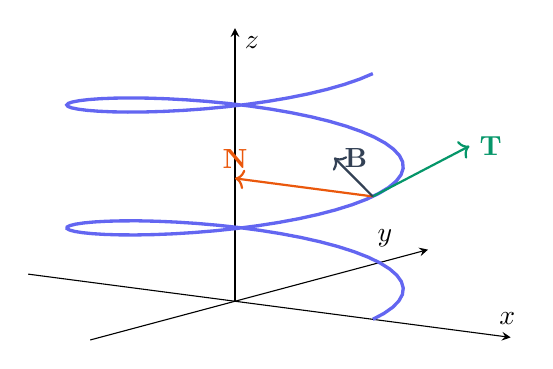
\begin{tikzpicture}\begin{axis}[width=12cm,height=7cm,view={35}{22},axis lines=center,xlabel=$x$,ylabel=$y$,zlabel=$z$,ticks=none,xmin=-1.5,xmax=2,ymin=-1.5,ymax=2,zmin=0,zmax=5]
\addplot3[very thick,blue,domain=0:720,samples=100,samples y=0]({cos(x)},{sin(x)},{x/160});
\addplot3[thick,->,green]coordinates{(1,0,2.25)(1,1,2.7)} node[pos=1,right]{$\mathbf T$};
\addplot3[thick,->,orange]coordinates{(1,0,2.25)(0,0,2.25)} node[pos=1,above]{$\mathbf N$};
\addplot3[thick,->,ink]coordinates{(1,0,2.25)(1,-.4,3.15)} node[pos=1,right]{$\mathbf B$};
\end{axis}\end{tikzpicture}
\end{document}
